\part*{}

\chapter{Schlussbetrachtungen} % (fold)
\label{cha:schlussbetrachtungen}

\begin{figure}[htbp]
	\centering
		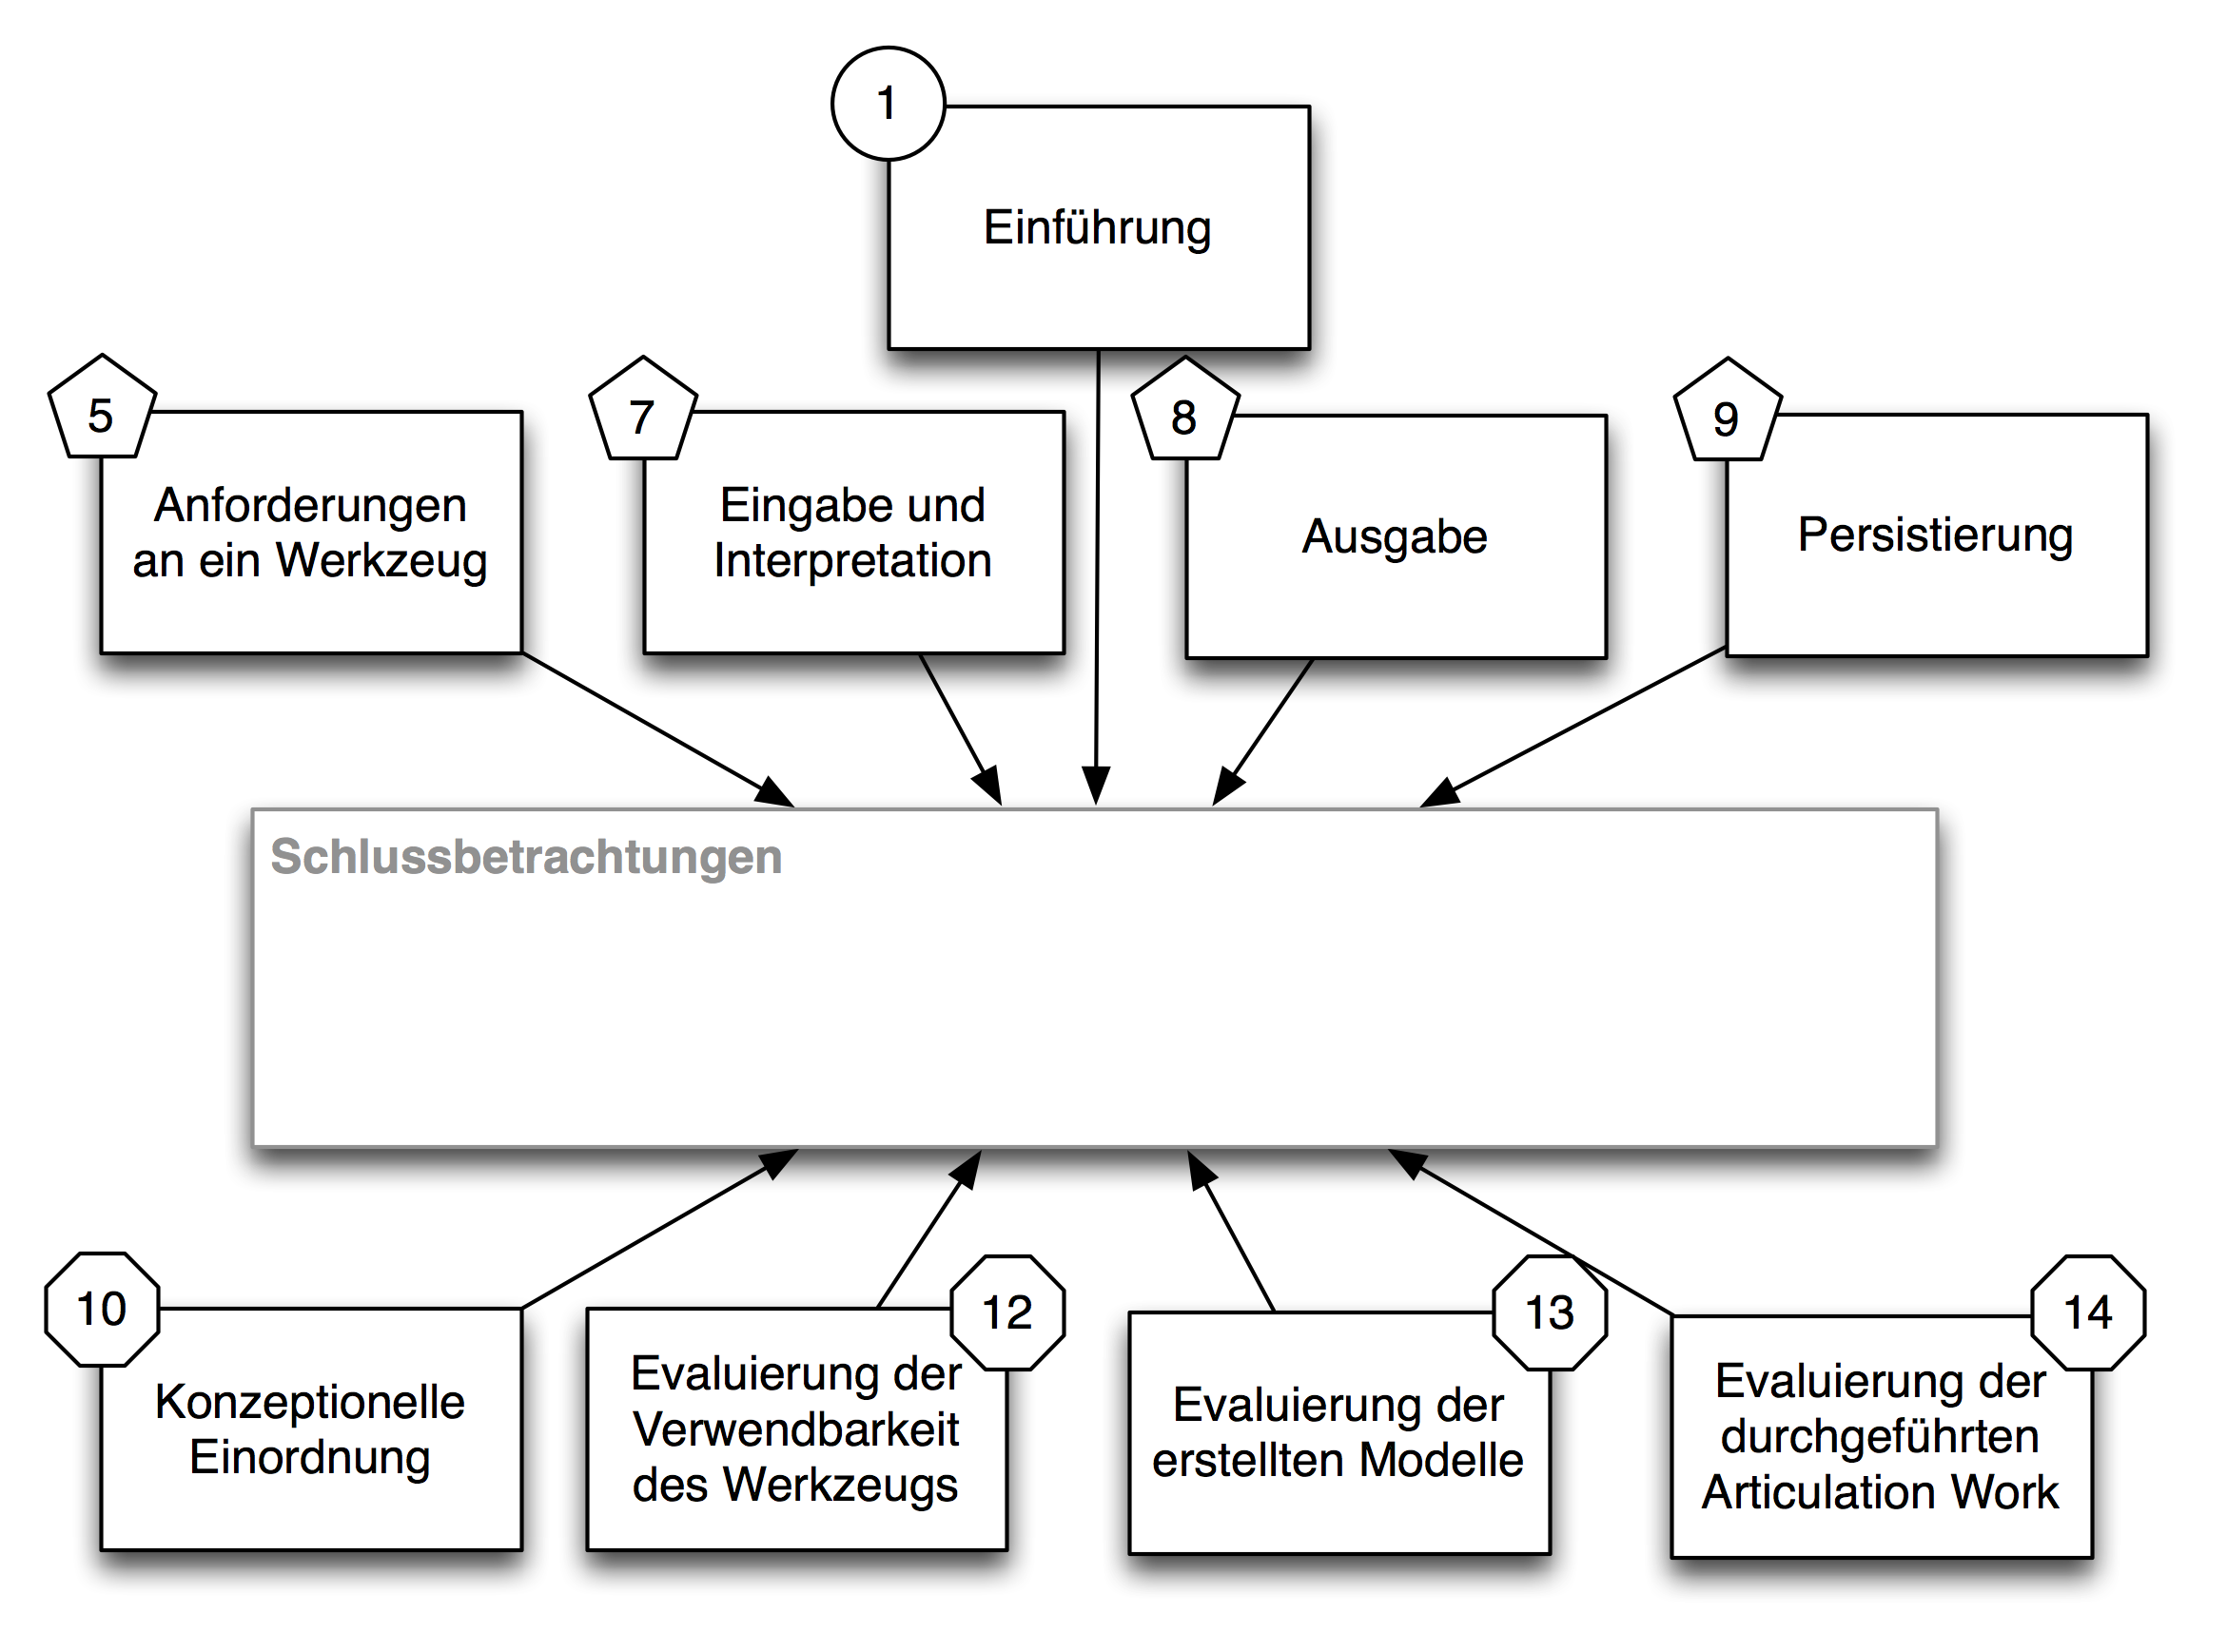
\includegraphics[scale=0.7]{img/Kontextgrafiken/k15.png}
	\caption{Kapitel „Schussbetrachtungen“ im Gesamtzusammenhang}
	\label{fig:img_Kontextgrafiken_k15}
\end{figure}

\section{Überblick über den Gesamtzusammenhang} % (fold)
\label{sec:überblick_über_den_gesamtzusammenhang}

\begin{figure}[htbp]
	\centering
		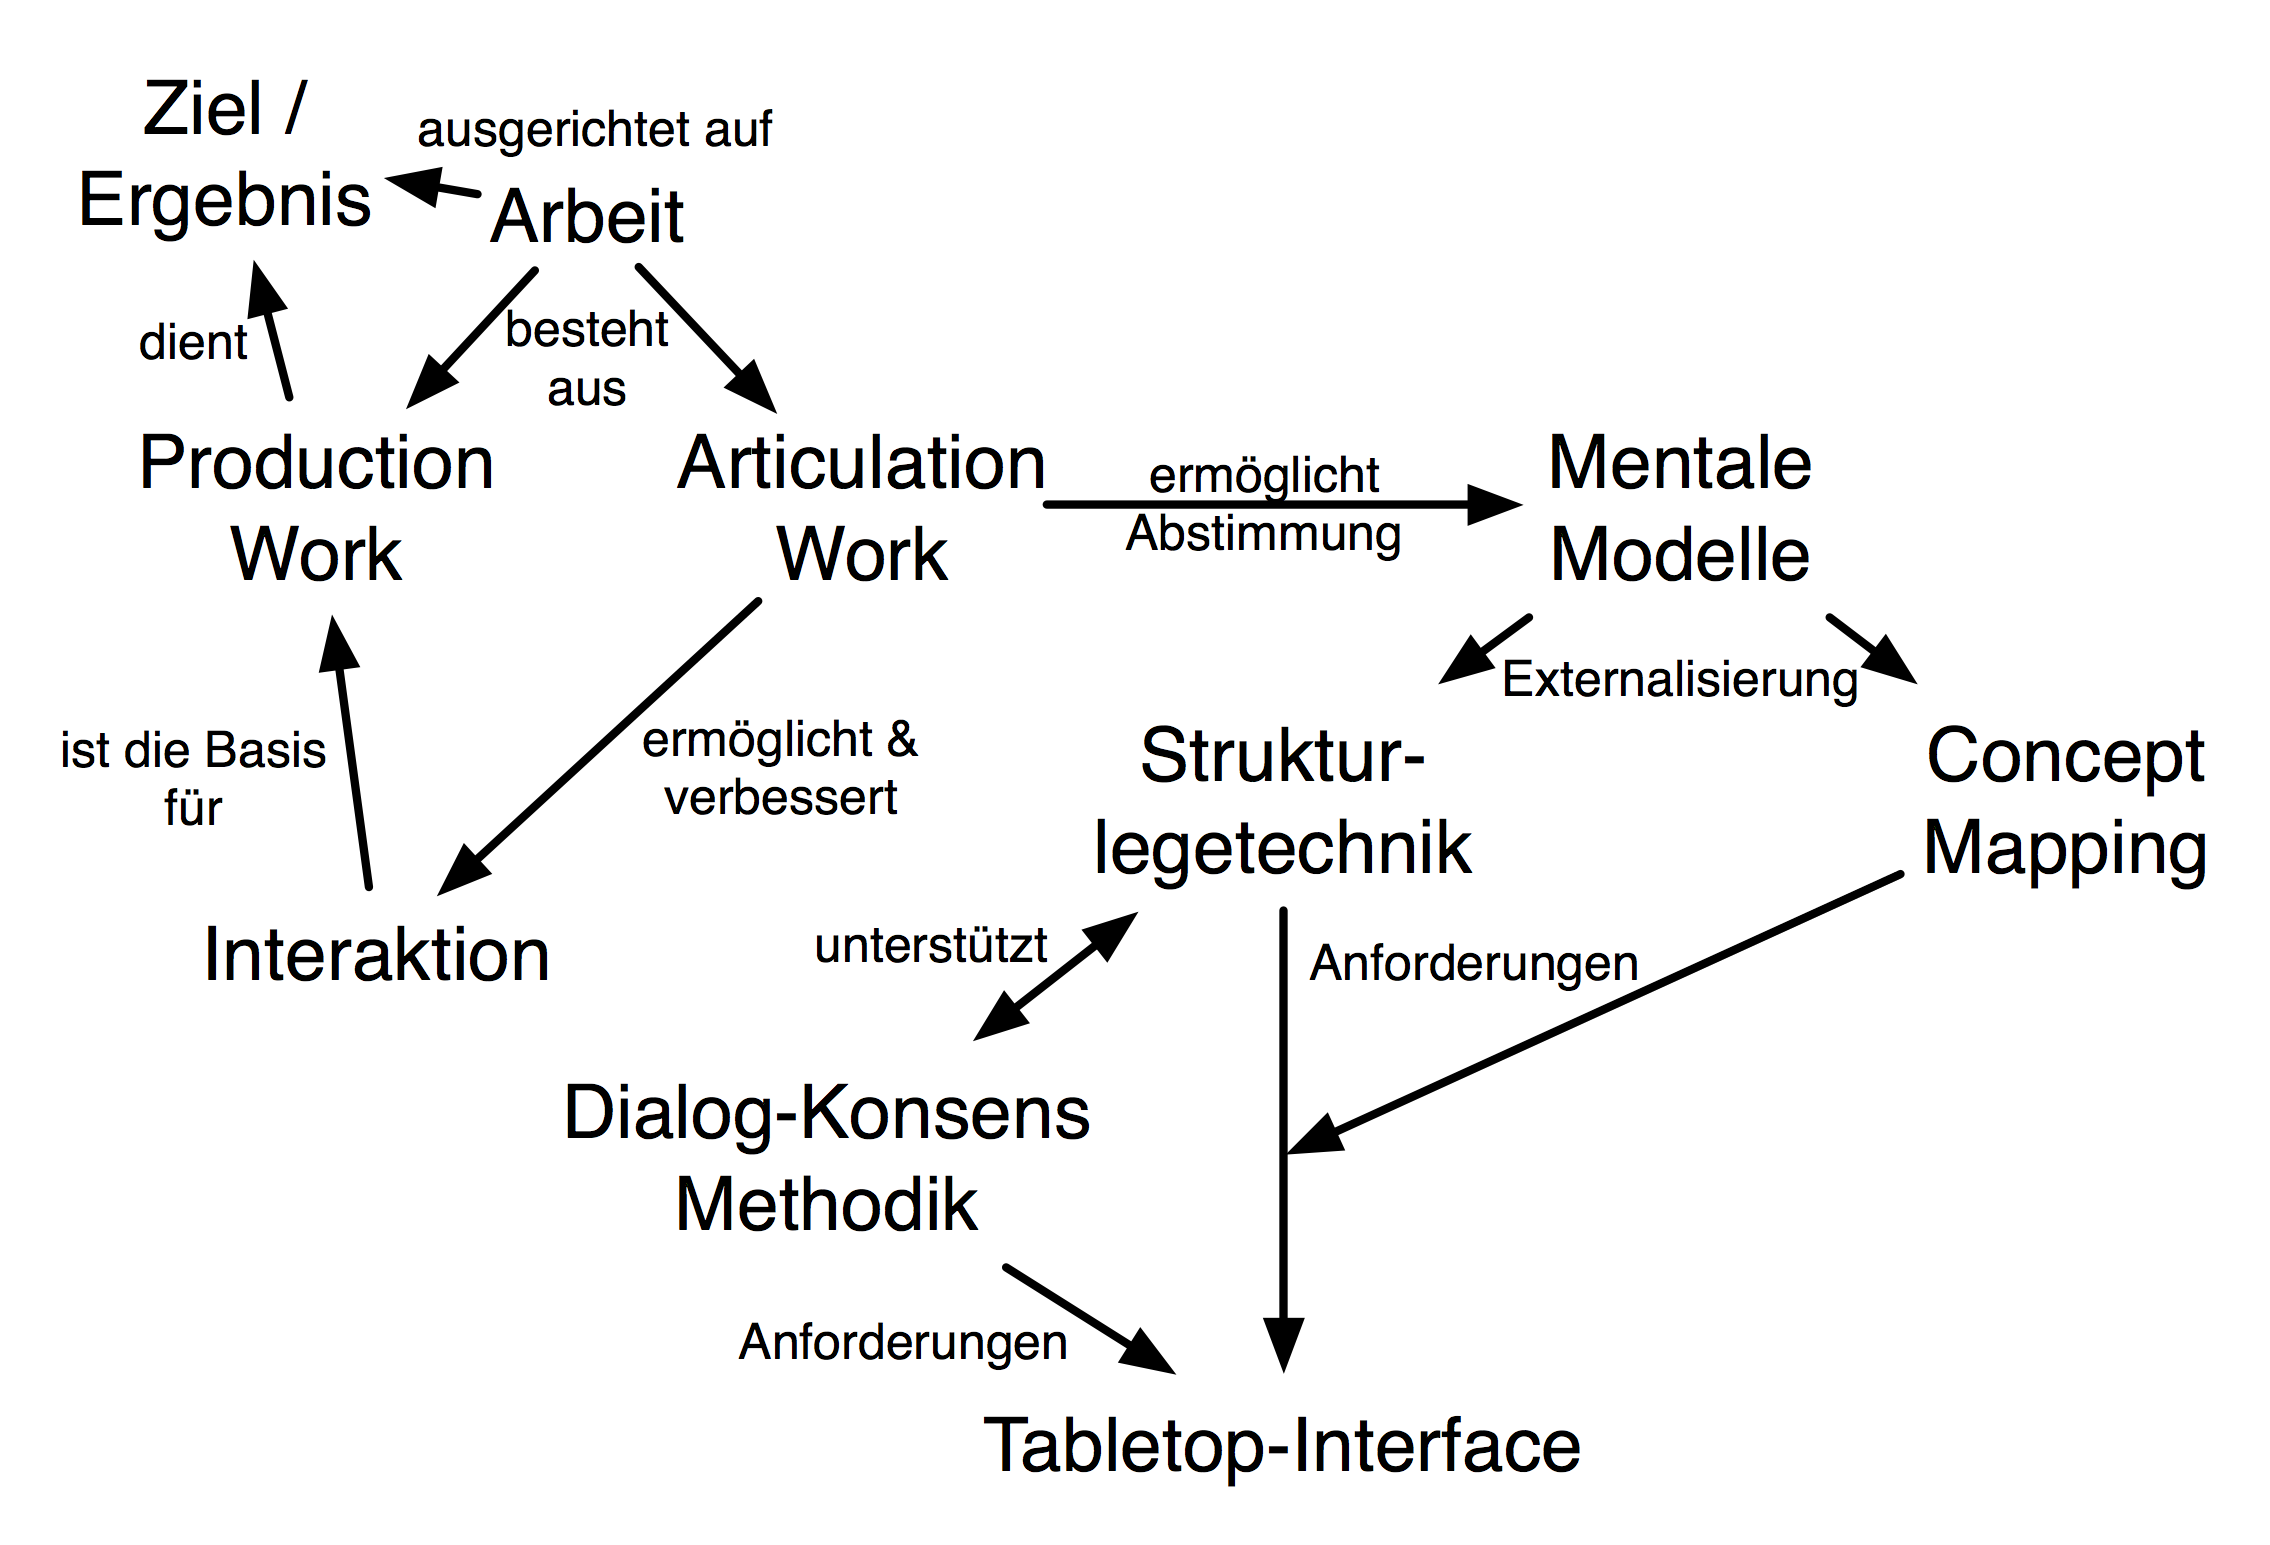
\includegraphics[width=10cm]{img/Schlussbetrachtungen/ArbeitInteraktionMentaleModelleTabletop.png}
	\caption{Gesamtzusammenhang der in dieser Arbeit verwendeten Konzepte}
	\label{fig:img_Schlussbetrachtungen_ArbeitInteraktionMentaleModelleTabletop}
\end{figure}

evtl. noch zweite Grafik, die die Kapitel der Arbeit in diese Struktur einordnet.

% section überblick_über_den_gesamtzusammenhang (end)

\section{Erfüllung der Anforderungen an das Werkzeug}

Hier rein: Zusammenfassung der Evaluierung. Aufhänger: Formulierte Anforderungen

\section{Bewertung hinsichlich der globalen Zielsetzung}

Hier rein: Ergebnis der Evaluierung hinsichtlich der globalen Zielsetzung

\section{Offene Aspekte und Entwicklungspotential}

noch offen

\section{Schluss}

hier rein: Schlussresümee

Hypothesen zeigen: Geeignet für Articulation Work, eher nicht geeignet für detaillierte Modellbildungen, technisch keine Probleme mehr.

Schlussfolgerung: Werkzeug unterstützt den Prozess der kommunikativen Abstimmung von mentalen Modellen, nicht aber die vollständige Externalisierung derselben.

% \section{Anwendungsszenarien} % (fold)
% \label{sec:anwendungsszenarien}
% 
% \subsection{Problembeschreibung und Arbeitsabstimmung}
% 
% Einzel- oder Gruppensessions. 
% 
% Aufgabenstellung: meist aus Arbeitsabläufen der beteiligten Personen
% 
% Merkmal: Tisch ist Mittel zum Zweck, gelegtes Modell fungiert als Diskussionsgrundlage. Modell ist statisch, wird einmal gelegt und nicht mehr verändert. Eher kompakte Modelle, die den Kontext eines Problems beschreiben. Die eigentliche Problematik ist selten explizit im Modell dargestellt.
% 
% Anwendungsbeispiele: Block 1, Block 2, Block 4 (Session 1-3).
% 
% Vorteile:
% 
% \subsection{Concept Mapping}
% 
% Einzel- oder Gruppensessions. 
% 
% Aufgabenstellung: zur Erhebung bzw. Überprüfung von domänenspezifischen (Struktur-)Wissen
% 
% Merkmal: Tisch 
% 
% Anwendungsbeispiele: Block 3, Block 5
% 
% \subsection{Strukturaufstellung und Manipulation}
% 
% Anwendungsbeispiele: Block 4 (Session 4).
% 
% AUfgabenstellung: Erhebung und Reflexion der Strukturen in denen Arbeitsabläufe situiert sind (Abteilungen, Personen, Kommunikationskanäle).
% 
% Merkmal: Modelle sind nicht statisch - werden nach der Erstellung zwar meist nicht erweitert aber in ihrer Struktur verändert (räumliche Relation der Knoten zueinander). 
% 
% % chapter schlussbetrachtungen (end)